%--- Chapter 5 ----------------------------------------------------------------% 
%\usepackage{siunitx}  %% BN: causes latex error

\chapter{Results and analysis} 
In this chapter, all possible results and metrics to evaluate the proposed framework, followed by its respective interpretations are provided. Final conclusions on the framework as a whole with its strengths and weaknesses are given in the conclusion chapter.  We will first look at evaluation metrics for predicting the execution time of parallel graph processing experiments followed by metrics for evaluating its respective classification. Lastly, we will discuss the evaluation metrics for predicting and ranking experiments a for system of linear equation. 
\section{Parallel graph processing experiments}
We have proposed solutions for two different classes of problems within graph processing experiments. The prediction problem is evaluated using three metrics, namely the $R^2$ value, Root-Mean Squared(RMSD) and Normalized Root-Mean Squared Deviations (NRMSD).
On the other hand, we will evaluate the classification problem on the number of false positive and negative predictions. This can be visualized using a confusion matrix. We will also introduce a new metric that measures the improvement from choosing the experimental setup provided by the framework.

\subsection{Execution time prediction}

\begin{figure*}
    \centering
    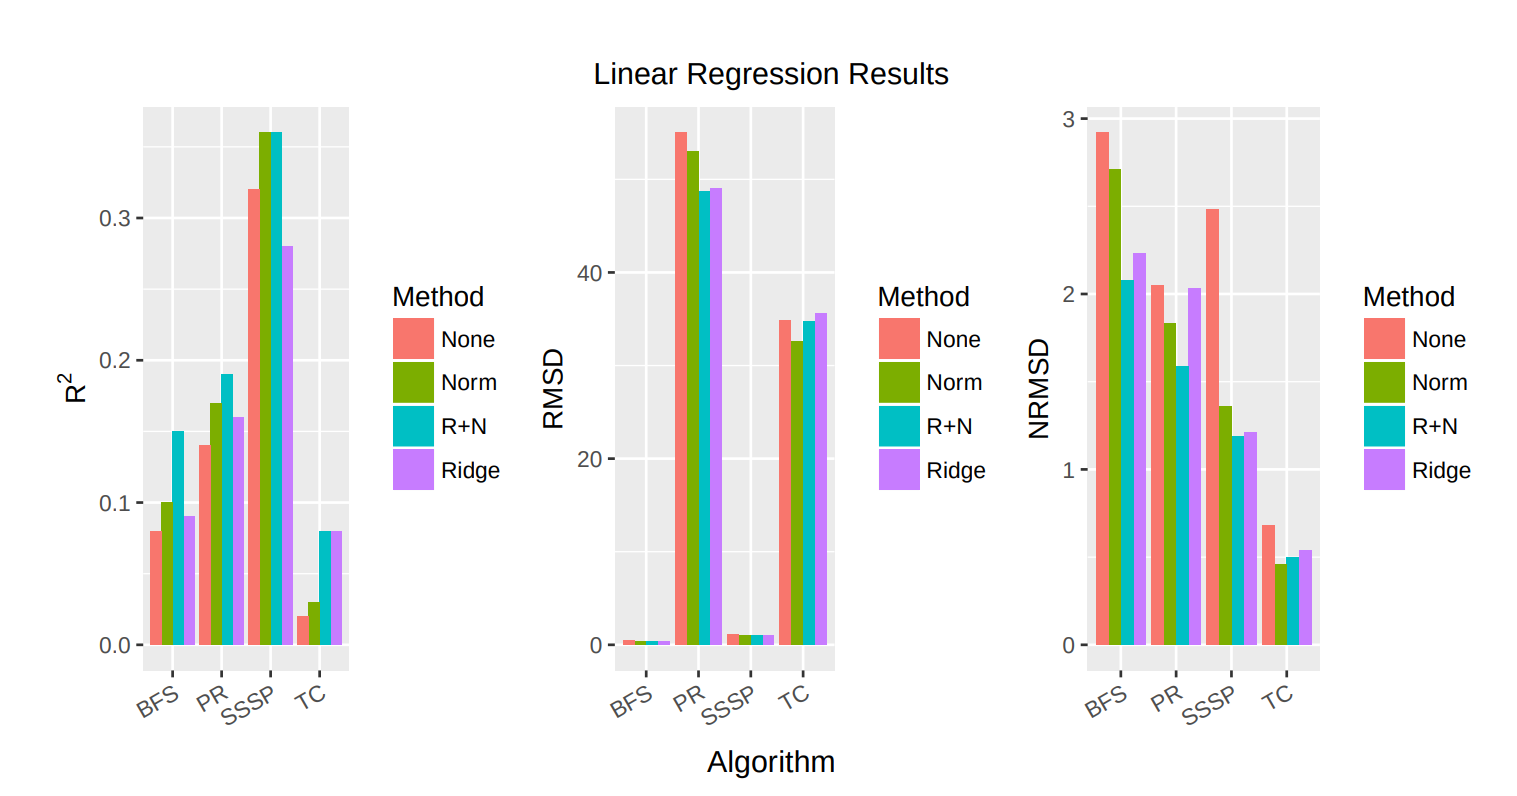
\includegraphics[width=1\columnwidth]{figures/regression_results.png}
    \caption{Linear regression with and without ridging and normalization}
    \label{Linear regression with and without ridging and normalization}
\end{figure*}

Figure \ref{Linear regression with and without ridging and nor-malization} shows us a consolidated comparison of all three metrics for each model configuration across four different algorithms. The $R^2$ value (left plot) signifies the goodness of fit in contrast to a mean model, which uses the mean for every predicted value. This is based on the observation that a well-fitting regression model results in predicted values close to the observed data values, and the proposed regression model should, therefore, be better than the fit of the mean model. It ranges from 0-1 with higher values indicating a better fit. 

On the other hand, RMSD(middle plot) measures the closeness of predicted values to the actual value. While $R^2$ is a relative measure of fit, RMSD is an absolute measure of fit. Lower values of RMSD signifies better fit. However, RMSD is hard to compare across algorithms. Algorithms like BFS has a much lower execution time compared to likes of TC. Thus, we use NRMSD(right plot).

It can be noted that for all algorithms across three metrics, the model configuration with ridge regression and normalized learning set is always best or at the very least tied for best. Although this configuration gives a significant improvement in the quality of predictions, it still isn't reliable enough to replace empirical models that run experiments rather than predicting them. Based on the size of our learning set, we must see  $R^2$ values above 0.7 for it to be considered a reliable replacement. 

Poor prediction performances can be attributed to the fact that execution times of experiments are minimal, specifically to the power of -5. To complicate this, the range of possible values is also quite big, ranging anywhere between the power of -2 and -5. This makes predictions more like finding a needle in a haystack.

\subsection{Classification of experiments}
The second model we propose in the framework is a classification model that aims to categorize a particular experiment as "good" or "bad" based on its traversed edges per second(TEPS).   

\begin{figure*}
    \centering
    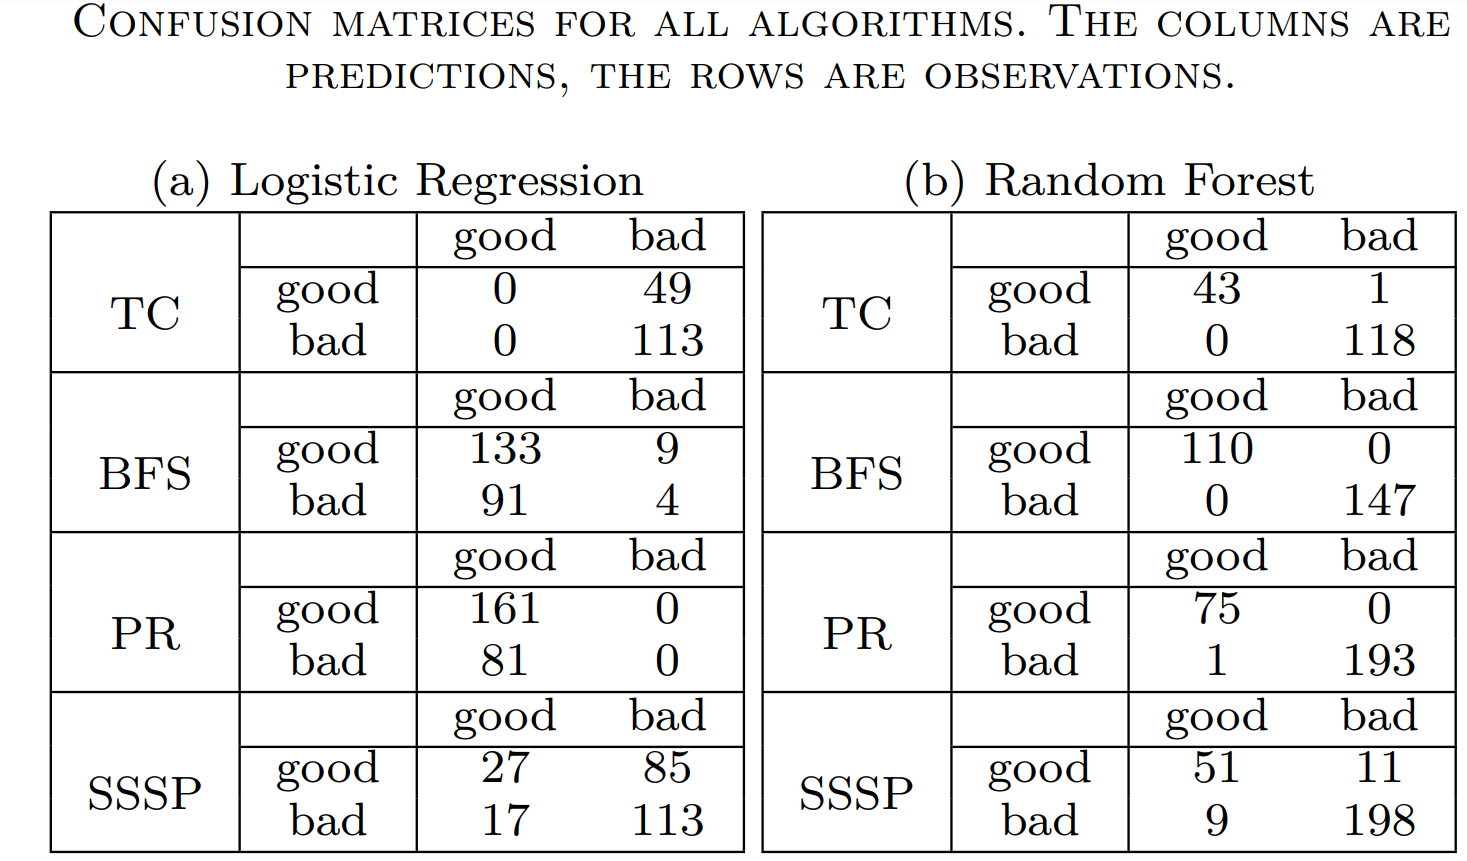
\includegraphics[width=1\columnwidth]{figures/classification_results.png}
    \caption{}
    \label{Confusion matrix}
\end{figure*}

Figure \ref{Confusion matrix} (b) gives us the confusion matrix for the random forest model and just for comparison, the confusion matrix for logistic regression in figure \ref{Confusion matrix} (a). The confusion matrix is used to measure the number of true and false positives and likewise, its negative counterpart. The rows indicate class labels from actual observations or ground truth while the columns indicate the class labels that were predicted by the models. For example, the random forest model predicted 44 different experiments that run TC to be good but turns out only 43 were observed to be good while the 1 experiment was actually bad. This means the model made 43 true positive predictions and one false positive prediction. Likewise, the model predicted 118 experiments to be bad, and indeed, all 118 experiments were actually observed to be bad. This means the model made 118 true negative predictions and 0 false negative predictions.

A general rule of thumb for well-performing models is to have confusion matrices with large leading diagonals and small non-leading diagonals. With that in mind, one can see that random forest performs exceptionally for TC, BFS, and PR with a maximum of one misplaced prediction from over 200 predictions. For SSSP though, the predictions aren't quite as spectacular but good nonetheless with 20 misplaced predictions. \todo{I have no idea why}

This gives us a \textbf{total testing accuracy of 97\%} across four algorithms. In comparison, one can see that logistic regression falls far behind with significant misplaced predictions. Apart from the overall count of misplaced predictions, the type of misplacement matters. Having more false positives is worse than having more false negatives as users don't mind having a few "good" experiments being termed "bad" resulting in them not using a package. But on the other hand, having "bad" experiments tagged as "good" leads them to go ahead and use a package and as a result cause significant slowdowns. It is important to note that the end objective of this framework is to provide reliable options for package selection, and having few false negatives is fine at the cost of minimal false positives.

Another metric we introduce to evaluate the performance of the classification model is \textbf{improvement}. This is mainly used to signify how much of performance improvement a user gets by choosing a "good" labeled experiment setup given by the framework rather than using any random experiment setup. Improvement can be defined as


\[
Improvement=  \frac{Mean(TEPS\;of\;data\;labeled\;as\;Good)}{Mean(TEPS\;of\;all\;data)}
\]
\vspace{4 pt}


\begin{figure*}
    \centering
    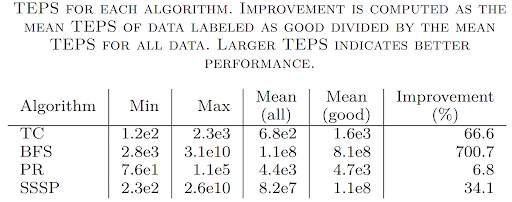
\includegraphics[width=1\columnwidth]{figures/classification_improvement.png}
    \caption{}
    \label{Improvement}
\end{figure*}

Figure \ref{Improvement} gives us the performance improvement along with the min, max, and mean across the four algorithms for the random forest model. It should be noted that larger TEPS value indicates better performance since it is a factor of execution time rather than its multiple. We can see that TC and SSSP have a good performance improvement while BFS tops the chart with a remarkable 700\% improvement. The performance improvement for PR is not as high as the other algorithms. The low variance explains this in execution time and TEPS of PR. The coefficient of variation (standard deviation/mean) of TEPS for BFS is 1.5, and PR is only 0.21. 

\section{Experiments on solving linear systems}
\todo{Always start with some text -- not going straight to a subsection.}

\subsection{Predicting execution times for experiments}
In this section, we will first discuss the results for predicting execution times of different experiments solving a system of linear equations. Once again, the three metrics, namely, $R^2$ values, root-mean-squared-deviation, and its normalized counterpart, are used for evaluating the prediction accuracy. From ***, you can see that the $R^2$ values are similar or even slightly worse compared to that of the graph processing application. This is once again because the data points are not linearly separable, and even a ridge regression model is not accurate enough. The RMSD and NRMSD values are slightly better with all test sets having values less than 0.8. 

With these results, we can say the predictions are not yet reliable enough. But a critical aspect that we can observe from the learning set is that the range of execution times across experiments is pretty big and ones that are considered good have far smaller times than the ones considered bad. As a result, there is a strong separation between them, even with the predictions. This was the key inspiration behind the proposed ranking algorithm. 

\subsection{Ranking experiments for linear systems}
This section will provide the ranking results for the two different learning sets we ran experiments on. The main metric we use to draw conclusions on is the speedup, which is given by:
\[
Speedup=  \frac{Time\;taken\;by\;baseline\;solver}{Time\;taken\;by\;\#1\;solver}
\]


This definition signifies the speedup in execution time one gets by choosing a solver recommended by our framework rather than choosing the default solver offered by PETSc, which is our baseline. To clarify, the speedup isn't actually from improving the solvers by themselves but rather from selecting better solvers for that particular linear system and its experimental setup. We will also discuss other metrics like average precision and reciprocal ranks to solidify our conclusions. 

\textbf{SuiteSparse Matrix Collection:}\\

As previously discussed, we have trained our model with a training set dominated by experiments labeled "good" and tested it across 1041 different linear systems with each having its own testing set dominated by experiments labeled "bad." From table \ref{Statistics of speedups across all testing sets}, we can see that even the minimum speedup is 1.14, which means the number one solver that the framework provides is better than the baseline solver for all the testing sets, which in this case is GMRES with Block Jacobi.\todo{background and cite kanika} In fact, the proposed solver is way better than the baseline solver with an average speedup of 746 and peaking at 92464 across all testing sets. 

\begin{figure*}
    \centering
    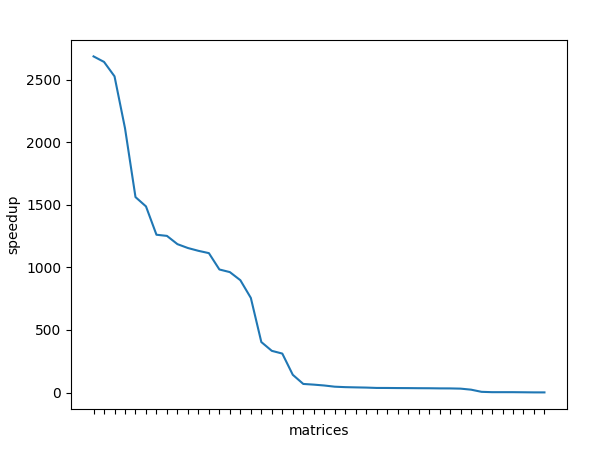
\includegraphics[width=1\columnwidth]{figures/speedup_graph.png}
    \caption{spread of speedups across testing sets}
    \label{spread of speedups across testing sets}
\end{figure*}

Figure\ref{spread of speedups across testing sets}, shows us the spread of speedups across 100 randomly chosen testing sets(linear systems). The x-axis denotes all the systems in decreasing order of execution time while y-axis indicates the speedup. We can note that speedups decrease in proportion to the execution time. This can be attributed to the fact that the prediction accuracy of our ridging model also decreases with execution time, and as a result, the proposed rank positions are way off from their actual rank positions. But considering speedups alone can be misleading. 



\begin{table}
\centering
\caption{Statistics of speedups across all testing sets}
\label{Statistics of speedups across all testing sets}
\begin{tabular}{|c|c|c|}    \hline  

speedup stats                                 & Values\\ \hline\hline
Min                         & 1.14 \\ \hline
Max                                       & 92464  \\ \hline
Mean                                       & 746  \\ \hline
Standard deviation                                          & 37\\ \hline

\end{tabular}
\end{table}

As mentioned in the introduction, the objectives of the ranking framework is to not only attain better speedups but to also ensure reliability. Reliability here means always suggesting good solver selections. Average speedups amount to very little if at the end of the day, the user still has to use a bad solver for an experiment. The user is most likely to choose solvers in order of rank and we need to ensure there isn't a choice of bad solvers before good. Figure *** shows us the top 10 ranked list of solvers for 1 example test set. It could be seen that the \#1 and \#2 ranked solvers are indeed solvers labeled "good" followed by the rest of bad solvers. This trend has followed in all test sets where the \#1 ranked solvers are good. A good metric to signify this trend is Mean-Reciprocal-Rank (MRR). RR in general for a particular test set is given by : 

\[
RR=  \frac{1}{Highest\;rank\;of\;a\;good\;solver}
\]

 For example, from figure \ref{Top 10 ranked experiments}, we can see that the highest rank of a good solver is \#1 and as a result, it has a reciprocal rank of 1 which is the highest possible value. Had the good solver been placed at \#3, the RR would have a value of 1/3. The mean value of RR across all testing sets is MRR. The MRR value we got is again 1 which signifies that the predicted \#1 solver is never bad. This goes a long way in ensuring reliability.
 
 \begin{figure*}
    \centering
    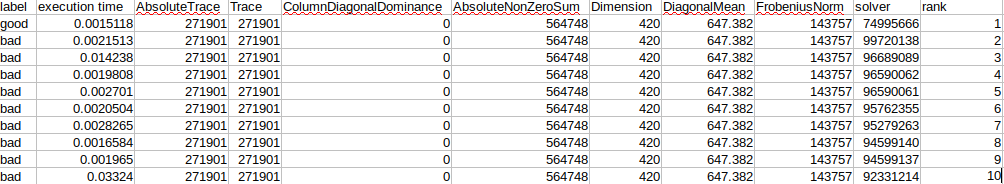
\includegraphics[width=1\columnwidth]{figures/rank_order.png}
    \caption{Top 10 ranked experiments}
    \label{Top 10 ranked experiments}
\end{figure*}

\textbf{MOOSE:}\\
Likewise, the experiments run on our second learning set also yielded similar results. For the model tested across 435 linear systems, table \ref{Statistics of speedups across all testing sets(MOOSE)} shows us the statistics of speedups across testing sets. Although the speedups are not as high as that of SuiteSparse Matrix Collection, it still follows the same trend of always having a positive speedup meaning, the \#1 ranked solver is always better than the baseline solver which in this case is GMRES with ILU, having a factor level of 0.\todo{background and cite kanika}. The relatively low speedup is mostly due to the smaller size of training set. From the table, we can also say that on an average, our recommended solver is 7 times faster than the baseline solver which PETSc offers, for any specific experiment setup.



\begin{table}
\centering
\caption{Statistics of speedups across all testing sets(MOOSE)}
\label{Statistics of speedups across all testing sets(MOOSE)}
\begin{tabular}{|c|c|c|}    \hline  

speedup stats                                 & Values\\ \hline\hline
Min                         & 1.2 \\ \hline
Max                                       & 857  \\ \hline
Mean                                       & 7.58  \\ \hline
Standard deviation                                          & 34\\ \hline

\end{tabular}
\end{table}